\chapter{Image processing using the graph Laplacian operator}

\paragraph{}
Multiple image processing filters can be built using the graph Laplacian operator.
As Milanfar mentions in \cite{siam_slides_2016} \cite{glide_2014} \cite{talebi_nonlocal_2014}, smoothing, deblurring, sharpening, dehazing, and other filters can be created.
Laplacian operators can also be used as the basis for compression artifact removal, low-light imaging and image segmentation.

We shall consider an adapted version of the proposed algorithm in \cite{glide_2014} to solve the eigenvalue problem by solving linear systems.
Let's introduce step-by-step the algorithm, the approximations and the possible variations.

\section{Algorithm}
\paragraph{}
A global image filter consists of a function which outputs one pixel, taking all pixels as input and applying weights to them.
\ifthesis
 Let \(z_i\) be the output pixel, \(W_{ij}\) the weights, \(y_j\) all input pixels and \(N\) the number of pixels in the image.
 We compute one output pixel with:
 \[z_i = \sum^{N}_{j=1} W_{ij}y_j,\]
 This means that a vector of weights exists for each pixel.
\fi

As a practical notation, we say that, with \(W\) the matrix of weights and \(y\) and \(z\) respectively the input and output images as vectors,
\[z = Wy.\]
The filter matrix \(W\) considered here is data-dependent and built upon the input image \(y\).
A more mathematical notation would consider \(W\) as a nonlinear function of the input image such as \(z = W(y) \cdot y\).


\paragraph{Image as graph}
Let's think of an image as a graph.
Each pixel is a node and has edges to other nodes.
The simplest way to connect pixels to other pixels is their direct neighbours, in which case each node has four edges.
To avoid losing any information, we will instead consider the case of a complete graph; each node connects to all other nodes.

To preserve the image information in the graph, the graph edges will be assigned a weight, measuring the similarity\footnote{Also called affinity.} between two nodes, thus between two pixels.

There are multiple ways the similarity can be defined.
The most intuitive definition considers spatial proximity.
This means that similar pixels are spatially close, which, translated to a basic filter, is the same as a Gaussian filter which computes a weighted average of the pixel's neighbourhood and produces what is known as Gaussian blur.
Another similarity definition is to consider the pixel's colour.
A good compromise is to consider an average of both, spatial and colour closeness, with a certain weighting.
\ifthesis
A summary of some affinity functions can be found in section \ref{variations:affinity_functions}.
\fi

Once the similarity is defined, we can compute the adjacency matrix of the graph including the edge weights.
This matrix is called the affinity matrix\footnote{Or similarity matrix, or kernel matrix}\ \(K\) which represents the similarity of each pixel to every other pixel in the image.
Consequently, this matrix is symmetric and of size \(N \times N\) with \(N\) the number of pixels in the image.
Also, most similarity functions define bounds on the values of \(K\) such as \(0 \le K_{ij} \le 1\).

Using this affinity matrix, we obtain the graph Laplacian \(\Lapl\), used to build the filter matrix \(W\).


\paragraph{Building the filter}
Multiple graph Laplacian definitions, more or less equivalent, exist and can have slightly different properties.
The table \ref{table:laplacians} proposes a summary of most Laplacian matrix definitions.
In the case of image smoothing, the filter \(W\) is roughly defined such as \(\Lapl = I - W\) \cite{siam_slides_2016} and so \(W = I - \Lapl\).
To get various filters using one Laplacian, we can apply some function \(f\) to \(\Lapl\) and obtain \(W = I - f(\Lapl)\) which gives us more possibilities on the filter computation.
Below the global filter algorithm if we compute the entire matrices:

\begin{algorithm}[H]
 \caption{Image processing using entire graph Laplacian operator}
 \begin{algorithmic}
  \REQUIRE \(y\) an image of size \(N\), \(f\) the function applied to \(\Lapl\)
  \ENSURE \(z\) the output image
  \STATE Compute \(K\) (size \(N \times N\))
  \STATE Compute Laplacian matrix \(\Lapl\)
  \STATE \(z \leftarrow (I - f(\Lapl)) y\)
 \end{algorithmic}
\end{algorithm}

However, all these matrices \(K\), \(\Lapl\) and \(W\) represent huge computational costs.
Only storing one of these matrices is already a challenge since they have a size of \(N^2\).

For example, a tiny test image of size \(256 \times 256\) has 65 536 pixels, so one of these matrices has approximately \(4.29 \times 10^9\) elements.
Considering storing those with a 64 bits type, one matrix takes more than 34 GB of memory.
Scaling to an everyday-smartphone picture, taken with a 10 MPixel camera, a matrix contains \(10^{14}\) elements, meaning 800 TB of memory for each matrix.


\paragraph{Approximation by sampling and Nystr\"om extension}
To avoid storing any of those huge matrices, approximation will be necessary.
Following \cite{fowlkes_spectral_2004}, we define the Nystr\"om extension.
It starts by sampling the image and only select a subset of \(p\) pixels, with \(p \ll N\).
Numerically, \(p\) should represent around 1\% or less of the image pixels.
\ifthesis
 The rows and columns of a matrix \(K\) are reorganised such as \(K_A\) the upper left affinity matrix of \(K\) of size \(p \times p\), measuring the affinities between the sampled pixels.
 The submatrix \(K_B\) is holding the similarities between the sampled pixels and the remaining pixels and is of size \(p \times (N-p)\).
 And the lower right submatrix \(K_C\) contains the affinities between the remaining pixels.
 We have:
 \[K = \begin{bmatrix}K_A & K_B \\ K_B^T & K_C\end{bmatrix}.\]
 Knowing that \(K_C\) is of size \((N-p) \times (N-p)\) and that \(p \ll N\), this submatrix is still huge and must be avoided.
 
 To have a numerical approximation of a symmetric (semi) positive definite matrix \(K\), we use the eigendecomposition with \(\Phi\) the orthonormal eigenvectors of \(K\) stored as a matrix and \(\Pi\) the eigenvalues of \(K\):
 \[K = \Phi \Pi \Phi^T.\]
 The article \cite{fowlkes_spectral_2004} suggests the Nystr\"om extension to approximate \(K\) by \(\tilde{K} = \tilde{\Phi} \tilde{\Pi} \tilde{\Phi^T}\), using the eigendecomposition of the submatrix \(K_A = \Phi_A \Pi_A \Phi_A^T\), with \(\tilde{\Pi} = \Pi_A\) and the approximated leading eigenvectors \(\tilde{\Phi}\):
 \begin{equation}
  \begin{split}
   \tilde{\Phi} & = \begin{bmatrix}\Phi_A \\ K_B^T K_A^{-1} \Phi_A \end{bmatrix} \\
                & = \begin{bmatrix}\Phi_A \\ K_B^T \Phi_A \Pi_A^{-1} \end{bmatrix}
  \end{split}
 \end{equation}
 We can calculate
 \begin{equation}
  \begin{split}
      \tilde{K} & = \tilde{\Phi} \tilde{\Pi} \tilde{\Phi^T} \\
                & = \begin{bmatrix} \Phi_A \\ K_B^T \Phi_A \Pi_A^{-1} \end{bmatrix} \Pi_A \begin{bmatrix} \Phi_A^T & \Pi_A^{-1} \Phi_A^T K_B \end{bmatrix} \\
                & = \begin{bmatrix} \Phi_A \Pi_A \\ K_B^T \Phi_A \end{bmatrix} \begin{bmatrix} \Phi_A^T & \Pi_A^{-1} \Phi_A^T K_B \end{bmatrix} \\
                & = \begin{bmatrix} K_A & K_B \\ K_B^T & K_B^T K_A^{-1} K_B \end{bmatrix}
  \end{split}
 \end{equation}
 
 We can clearly see that the huge submatrix \(K_C\) is now approximated by \(K_B^T K_A^{-1} K_B\).
 The quality of the approximation is measurable by the norm of the difference of the two above terms.
 We recognise the norm of the Schur complement \(\| K_C - K_B^T K_A^{-1} K_B \| \).
\else
 We only need to compute of subset of the affinity matrix \(K\) and then compute the eigendecomposition of a submatrix.
 The eigenvectors of the submatrix are extended to the entire matrix and used to reconstruct it.
\fi

Therefore, we will only need to compute two submatrices.
\ifthesis
 For our previous examples, if we sample 1\% of the pixels, we need to store 0.34 GB of data for each matrix, instead of 34 GB for the \(256 \times 256\) image.
 For a 10 megapixel image, each matrix needs 8 TB of memory, which is still a lot of memory.
 However, as \cite{fowlkes_spectral_2004} and \cite{glide_2014} propose, the sampling rate can be lower than 1\% and still contain most of the relevant image information.
\else
 For our previous example, for the 10 megapixel image, each matrix needs 8 TB of memory, which is still a lot of memory, but the sampling rate can be lower than 1\% as suggested by \cite{fowlkes_spectral_2004} and \cite{glide_2014}.
\fi


\paragraph{Eigendecomposition}
We need to compute the largest eigenvalues of the filter \(W\).
The reason can be found by formulating the filter by its diagonalisation \(W = \sum_i^N \lambda_i \phi_i \phi_i^T\).
When the \(i\)th eigenvalue \(\lambda_i\) is small, the eigenvector product will be negligible, and therefore the largest eigenvalues of the filter \(W\) are the most relevant.

For the approximation, we will actually need to compute the largest eigenvalues of the sampled pixels submatrix \(W_A\) to use the Nystr\"om extension.
Using a sample to compute the largest eigenvalues works to approximate the complete filter because these eigenvalues are decaying rapidly as shows the figure below:
\begin{figure}[H]
  \centering
  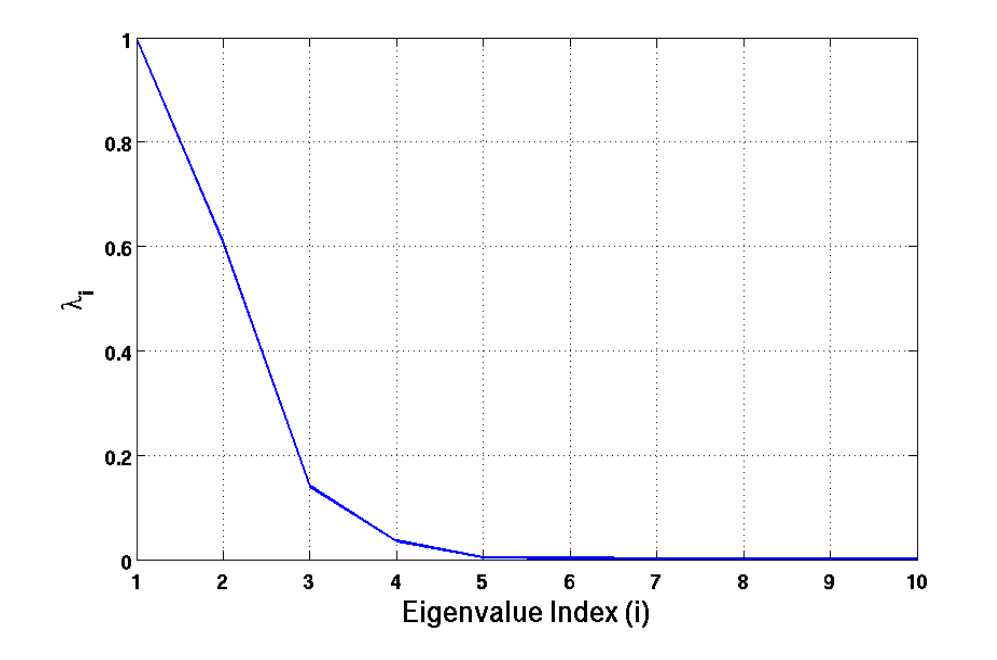
\includegraphics[width=0.9\textwidth]{img/decayingEigenvalues.png}
  \caption{Largest eigenvalues of an image filter, taken from \cite{siam_slides_2016}.}
\end{figure}
% TODO refaire soit meme

We know that the eigenvalues of submatrix\ \(W_A\) are between the extremum eigenvalues of the filter \(W\), which is known as the interlacing property of principal submatrices.
We also know that computing the largest eigenvalues of the submatrix filter is equivalent to computing the smallest eigenvalues of the corresponding Laplacian operator.
The proofs to these statements can be found in Appendix \ref{appendix:eigenvalue_proof}.

The goal of this observation is the way of computing the eigenvalues.
For the largest eigenvalues, the most famous algorithm is the power method.
For the smallest eigenvalues, the inverse power method is a usual choice.
Both methods converge faster when two successive eigenvalues are far from each other.
In our case, the largest eigenvalues are close to each other; hence the inverse of these eigenvalues will be far from each other.
We will therefore prefer the inverse power method.

The algorithm will, in an iterative manner, compute the associated eigenvector of an eigenvalue.
This requires either to invert a matrix such as \(x_{k+1} = A^{-1} x_k\), or to solve the linear system \(A x_{k+1} = x_k\).
We will solve systems of linear equations to compute the first eigenvalues of the Laplacian in order to observe the behaviour of solvers on these dense matrices.

The main drawback of the Nystr\"om method for us, is that it approximates the leading eigenvalues and we compute the trailing ones of the Laplacian \(\Lapl\) \cite{belongie_spectral_2002}.
It is possible to obtain the eigendecomposition of the filter \(W\), even when \(W\) is indefinite, through a method proposed by \cite{fowlkes_spectral_2004}.
It consists of computing the matrix \(W_A^{-1/2}\), which could be done either by the complete eigendecomposition or by using Cauchy's integral formula.
After this step, two more diagonalisation of matrices are required, demanding an important computation time.

Nevertheless, as stated in the objectives of the project, our main goal is not the image processing aspect, but the behaviour of linear solvers of these dense matrices using domain decomposition methods.
We will therefore stick to computing the smallest eigenvalues of the Laplacian operator \(\Lapl\) and avoid spending too much time on the end of the algorithm implementation.


\paragraph{}
As the size of the image grows, computing the first \(p\) eigenvalues can easily represent computing more than thousand eigenvalues since we consider 1\% of all pixels for the sampling step.
Instead, we define \(m\), with \(m \le p\), the number of computed eigenvalues of \(\Lapl_A\).
It is not required to compute all eigenvalues of the sampled pixels matrix, only the first ones are the most relevant, since they correspond to the largest eigenvalues of the filter.


\paragraph{Output image}
\ifthesis
 Even if we cannot approximate the trailing eigenvectors of \(\Lapl\) through the eigenvectors of \(\Lapl_A\), we still define how the Laplacian is used to compute the output image.
 The summary \cite{modern_tour_2013} implicitly defines the filter as \(W = I - f(\Lapl)\) with the function \(f\) that helps achieving various filters.
 To apply the function efficiently to the Laplacian operator, we apply it to the diagonal eigenvalue matrix such as \(f(\Lapl) = \Phi f(\Pi) \Phi^T\).
 The output image using the filter approximation \(\tilde{W}\) can be expressed as:
 \begin{equation}
  \begin{split}
      \tilde{z} & = \tilde{W}y \\
                & = (I - f(\tilde{\Lapl})) y \\
                & = (I - \tilde{\Phi} f(\tilde{\Pi}) \tilde{\Phi^T}) y \\
                & = y - \tilde{\Phi} f(\tilde{\Pi}) \tilde{\Phi^T} y
  \end{split}
 \end{equation}
\fi

Below a summary of the complete algorithm using spectral decomposition of the matrix to approximate it:

\begin{algorithm}[H]
 \caption{Image processing using approximated graph Laplacian operator}
 \begin{algorithmic}
  \REQUIRE \(y\) an image of size \(N\), \(f\) the function applied to \(\Lapl\)
  \ENSURE \(\tilde{z}\) the output image by the approximated filter
  \STATE \COMMENT{Sampling}
  \STATE Sample \(p\) pixels, \(p \ll N\)
  \STATE \COMMENT{Kernel matrix approximation}
  \STATE Compute \(K_A\) (size \(p \times p\)) and \(K_B\) (size \(p \times (N-p)\))
  \STATE Compute the Laplacian submatrices \(\Lapl_A\) and \(\Lapl_B\)
  \STATE \COMMENT{Eigendecomposition}
  \STATE Compute the \(m\) smallest eigenvalues \(\Pi_A\) and the associated eigenvectors \(\Phi_A\) of \(\Lapl_A\)
  \STATE \COMMENT{Nystr\"om extension and compute the filter}
  \STATE See methods of solution proposed by \cite{fowlkes_spectral_2004}
  \STATE \(\tilde{z} \leftarrow \tilde{W} y\)
 \end{algorithmic}
\end{algorithm}


\section{Variations}
\paragraph{}
Multiple steps in this algorithm are to be defined in concrete terms to implement them.
For each, several methods exist, with different properties.
We present some of these methods for the sampling, computing similarities and the Laplacian operator.

\subsection{Sampling method}

\paragraph{}
The sample requires to represent only less than 1\% of the pixels of the image \cite{fowlkes_spectral_2004}.
To achieve this, we can use different approaches.
The chosen method is decisive for the application of the Nystr\"om method.
It should capture a snippet of all relevant information in the image.
\begin{description}[align=left]
 \item [Random sampling (RS)] most common and simple sampling scheme, but no deterministic guarantee of the output quality. It can produce good results for images with poor resolution, but with a huge amount of data, random sampling is limited because it cannot reflect the structure of the data set \cite{zhan_improved_2017}.
 \item [K-means sampling (KS)] associate to each pixel a 5-D space (R, G, B, X, Y) and divide the pixels into K clusters (K centres). These clusters are a good sampling scheme for images with simple and uniform backgrounds \cite{kao_sampling_2012} \cite{zhang_improved_2008}.
 \item [Uniform spatially sampling] the uniformity of the sample gives good results for image sampling because of the spatial correlation of pixels. This method remains simple but effective \cite{glide_2014}.
  \begin{figure}[H]
      \centering
      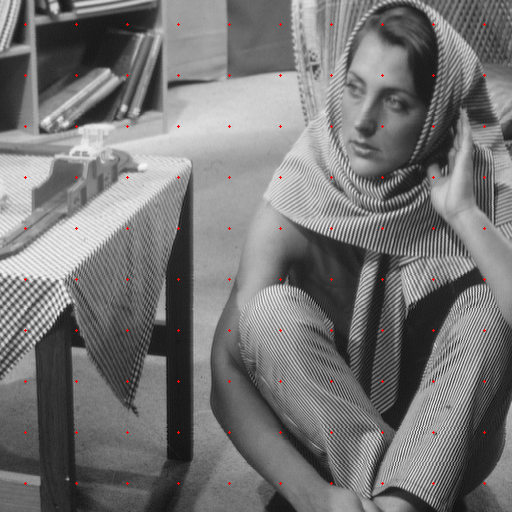
\includegraphics[width=0.6\textwidth]{img/spatiallyUniformSampling.png}
      \caption{Spatially uniform sampling. Red pixels are sampled. Here 100 pixels are sampled, which only represents 0.04\% of all pixels.}
  \end{figure}
 \item [Incremental sampling (INS)] is an adaptive sampling scheme, meaning that it select points according to the similarity, so that we can have an approximate optimal rank-k subspace of the original image \cite{zhan_improved_2017}.
 \item [Mean-shift segmentation-based sampling] this scheme performs good for complex backgrounds. The method consists in over-segmenting the image into \(n\) regions and only one pixel of each region will be sampled using the spatially closest pixel to the centre of the region given a formula in \cite{kao_sampling_2012}.
\end{description}

\subsection{Affinity function}
\label{variations:affinity_functions}

\paragraph{}
The kernel function measures the similarity between the pixel \(y_i\) and \(y_j\).
The chosen function is important because it decides on which features the similarity of pixels will be evaluated.
Some of the most used affinity functions are:

\begin{description}[align=left]
 \item [Spatial Gaussian kernel] takes only into account the spatial distance between two pixels \cite{siam_slides_2016}.
  The formula of this kernel is, with \(\forall i, j \in [1, N]\), \(x_i\) the coordinate vector of a pixel and \(h_x\) a normalisation parameter,
  \[K(y_i, y_j) = exp(-\frac{||x_i - x_j||^2}{h_x^2}).\]
  The parameter is influencing on the normalisation of the values and Gaussian standard deviation.
  The greater it is, the more tolerant the spatial distance computation will be.

 \item [Photometric Gaussian kernel] considers the intensity and colour similarity of the pixels \cite{siam_slides_2016}.
  The formula of this kernel is, with \(z_i\) the colour or grayscale of a pixel,
  \[K(y_i, y_j) = exp(-\frac{||z_i - z_j||^2}{h_z^2}).\]
  Generally, the \(h\) parameter is a smoothing parameter.
  If \(h\) is small, it is more discriminating between the affinity of different pixels.

 \item [Bilateral kernel] one of the most used kernel which smooths images by a nonlinear combination of the spatial and photometric Gaussian kernels \cite{siam_slides_2016} \cite{glide_2014} \cite{bilateral_tomasi_1998}:
  \[K(y_i, y_j) = exp(-\frac{||x_i - x_j||^2}{h_x^2}) \cdot exp(-\frac{||z_i - z_j||^2}{h_z^2}).\]

  To generate the example below, we use the famous grayscale image of Barbara of size \(512 \times 512\) pixels.
  The more a pixel is coloured in red, the more similar it is to the selected pixel, with respect to the chosen bilateral kernel.
  A blue coloured pixel is dissimilar to the considered pixel.
  These are two affinity vectors; the first one is of a pixel on the table leg and the second around Barbara's eye.
  Keep in mind that each affinity image shown represents only one row of the affinity matrix\ \(K\).

  \begin{figure}[H]
      \centering
      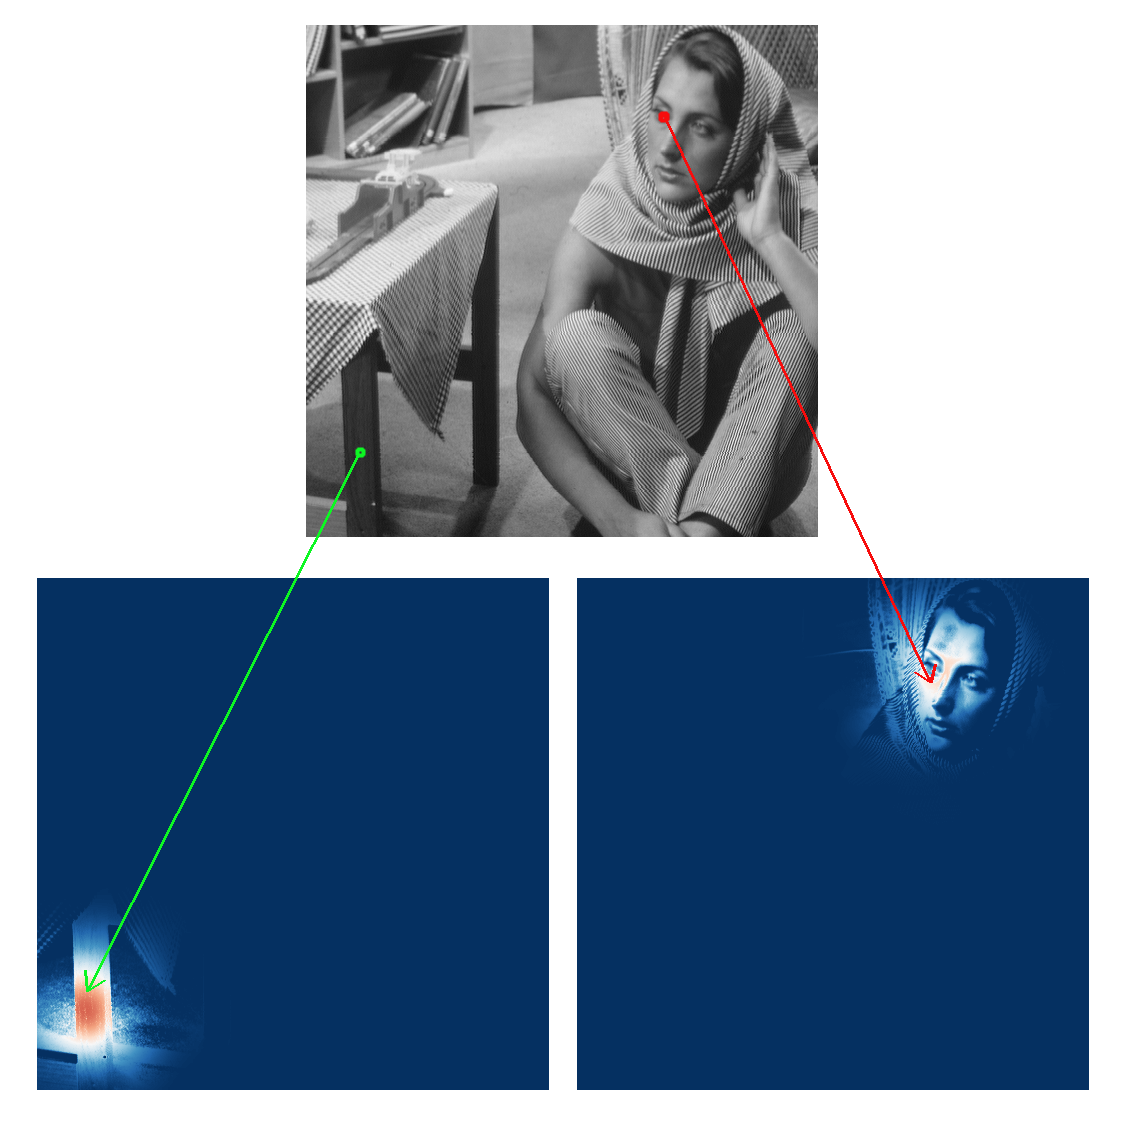
\includegraphics[width=\textwidth]{img/bilateralAffinityPhoto35Spatial50.png}
      \caption{Affinity matrices with \(h_x = 50\) and \(h_z = 35\).}
  \end{figure}
  In a very heterogeneous image, the bilateral kernel will be useful to keep the spatial similarity, but with excluding very dissimilar neighbour pixels.

 \item [Non-local means (NLM)] is similar to the bilateral kernel, a data-dependent filter, except that the photometric affinity is captured patch-wise \cite{glide_2014} \cite{kervrann_nlm_2006}.
 \item [Locally adaptive regression kernel (LARK)] uses the geodesic distance based on estimated gradients \cite{milanfar_symmetrizing_2013} \cite{takeda_kernel_2007}.
\end{description}

\subsection{Graph Laplacian operator}

\paragraph{}
The graph Laplacian operator has multiple possible definitions and each has its own properties.
A good summary can be found in \cite{siam_slides_2016} and \cite{chung_spectral_1997}.
A graph Laplacian can be symmetric which is important for the eigendecomposition of the matrix.
The spectral range, corresponding to the range of the eigenvalues, is important because we can use the filters derived from the Laplacian multiple times, and if the eigenvalues are not between 0 and 1, then the filters tend to be unstable.
With \(K\) being the affinity matrix, \(d_i = \sum_j K_{ij}\) and \(D = diag\{d_i\}\):

\begin{table}[!htbp]
 \centering
 \begin{tabular}{|c|c|c|c|c|}
  \hline
  Laplacian Name & Formula of \(\Lapl\) & Symmetric & Spectral Range \\
  \hline
  Un-normalised & \(D - K\) & Yes & [0, n] \\
  \hline
  Normalised & \(I - D^{-1/2}KD^{-1/2}\) & Yes & [0, 2] \\
  \hline
  Random walk & \(I - D^{-1}K\) & No & [0, 1] \\
  \hline
  ``Sinkhorn'' \cite{milanfar_symmetrizing_2013} & \(I - C^{-1/2}KC^{-1/2}\) & Yes & [0, 1] \\
  \hline
  Re-normalised \cite{milanfar_new_2016} & \(\alpha(D - K)\), \(\alpha = \bigO(N^{-1})\) & Yes & [0, n] \\
  \hline
 \end{tabular}
 \caption{Overview of different graph Laplacian operator definitions}
 \label{table:laplacians}
\end{table}
Generally, it is a good practice to stick to one definition of the Laplacian.

